% Options for packages loaded elsewhere
\PassOptionsToPackage{unicode}{hyperref}
\PassOptionsToPackage{hyphens}{url}
%
\documentclass[
]{book}
\usepackage{amsmath,amssymb}
\usepackage{lmodern}
\usepackage{iftex}
\ifPDFTeX
  \usepackage[T1]{fontenc}
  \usepackage[utf8]{inputenc}
  \usepackage{textcomp} % provide euro and other symbols
\else % if luatex or xetex
  \usepackage{unicode-math}
  \defaultfontfeatures{Scale=MatchLowercase}
  \defaultfontfeatures[\rmfamily]{Ligatures=TeX,Scale=1}
\fi
% Use upquote if available, for straight quotes in verbatim environments
\IfFileExists{upquote.sty}{\usepackage{upquote}}{}
\IfFileExists{microtype.sty}{% use microtype if available
  \usepackage[]{microtype}
  \UseMicrotypeSet[protrusion]{basicmath} % disable protrusion for tt fonts
}{}
\makeatletter
\@ifundefined{KOMAClassName}{% if non-KOMA class
  \IfFileExists{parskip.sty}{%
    \usepackage{parskip}
  }{% else
    \setlength{\parindent}{0pt}
    \setlength{\parskip}{6pt plus 2pt minus 1pt}}
}{% if KOMA class
  \KOMAoptions{parskip=half}}
\makeatother
\usepackage{xcolor}
\IfFileExists{xurl.sty}{\usepackage{xurl}}{} % add URL line breaks if available
\IfFileExists{bookmark.sty}{\usepackage{bookmark}}{\usepackage{hyperref}}
\hypersetup{
  pdftitle={MBAn Career Handbook Group Project Proposal},
  pdfauthor={Team Keep Rolling},
  hidelinks,
  pdfcreator={LaTeX via pandoc}}
\urlstyle{same} % disable monospaced font for URLs
\usepackage{color}
\usepackage{fancyvrb}
\newcommand{\VerbBar}{|}
\newcommand{\VERB}{\Verb[commandchars=\\\{\}]}
\DefineVerbatimEnvironment{Highlighting}{Verbatim}{commandchars=\\\{\}}
% Add ',fontsize=\small' for more characters per line
\usepackage{framed}
\definecolor{shadecolor}{RGB}{248,248,248}
\newenvironment{Shaded}{\begin{snugshade}}{\end{snugshade}}
\newcommand{\AlertTok}[1]{\textcolor[rgb]{0.94,0.16,0.16}{#1}}
\newcommand{\AnnotationTok}[1]{\textcolor[rgb]{0.56,0.35,0.01}{\textbf{\textit{#1}}}}
\newcommand{\AttributeTok}[1]{\textcolor[rgb]{0.77,0.63,0.00}{#1}}
\newcommand{\BaseNTok}[1]{\textcolor[rgb]{0.00,0.00,0.81}{#1}}
\newcommand{\BuiltInTok}[1]{#1}
\newcommand{\CharTok}[1]{\textcolor[rgb]{0.31,0.60,0.02}{#1}}
\newcommand{\CommentTok}[1]{\textcolor[rgb]{0.56,0.35,0.01}{\textit{#1}}}
\newcommand{\CommentVarTok}[1]{\textcolor[rgb]{0.56,0.35,0.01}{\textbf{\textit{#1}}}}
\newcommand{\ConstantTok}[1]{\textcolor[rgb]{0.00,0.00,0.00}{#1}}
\newcommand{\ControlFlowTok}[1]{\textcolor[rgb]{0.13,0.29,0.53}{\textbf{#1}}}
\newcommand{\DataTypeTok}[1]{\textcolor[rgb]{0.13,0.29,0.53}{#1}}
\newcommand{\DecValTok}[1]{\textcolor[rgb]{0.00,0.00,0.81}{#1}}
\newcommand{\DocumentationTok}[1]{\textcolor[rgb]{0.56,0.35,0.01}{\textbf{\textit{#1}}}}
\newcommand{\ErrorTok}[1]{\textcolor[rgb]{0.64,0.00,0.00}{\textbf{#1}}}
\newcommand{\ExtensionTok}[1]{#1}
\newcommand{\FloatTok}[1]{\textcolor[rgb]{0.00,0.00,0.81}{#1}}
\newcommand{\FunctionTok}[1]{\textcolor[rgb]{0.00,0.00,0.00}{#1}}
\newcommand{\ImportTok}[1]{#1}
\newcommand{\InformationTok}[1]{\textcolor[rgb]{0.56,0.35,0.01}{\textbf{\textit{#1}}}}
\newcommand{\KeywordTok}[1]{\textcolor[rgb]{0.13,0.29,0.53}{\textbf{#1}}}
\newcommand{\NormalTok}[1]{#1}
\newcommand{\OperatorTok}[1]{\textcolor[rgb]{0.81,0.36,0.00}{\textbf{#1}}}
\newcommand{\OtherTok}[1]{\textcolor[rgb]{0.56,0.35,0.01}{#1}}
\newcommand{\PreprocessorTok}[1]{\textcolor[rgb]{0.56,0.35,0.01}{\textit{#1}}}
\newcommand{\RegionMarkerTok}[1]{#1}
\newcommand{\SpecialCharTok}[1]{\textcolor[rgb]{0.00,0.00,0.00}{#1}}
\newcommand{\SpecialStringTok}[1]{\textcolor[rgb]{0.31,0.60,0.02}{#1}}
\newcommand{\StringTok}[1]{\textcolor[rgb]{0.31,0.60,0.02}{#1}}
\newcommand{\VariableTok}[1]{\textcolor[rgb]{0.00,0.00,0.00}{#1}}
\newcommand{\VerbatimStringTok}[1]{\textcolor[rgb]{0.31,0.60,0.02}{#1}}
\newcommand{\WarningTok}[1]{\textcolor[rgb]{0.56,0.35,0.01}{\textbf{\textit{#1}}}}
\usepackage{longtable,booktabs,array}
\usepackage{calc} % for calculating minipage widths
% Correct order of tables after \paragraph or \subparagraph
\usepackage{etoolbox}
\makeatletter
\patchcmd\longtable{\par}{\if@noskipsec\mbox{}\fi\par}{}{}
\makeatother
% Allow footnotes in longtable head/foot
\IfFileExists{footnotehyper.sty}{\usepackage{footnotehyper}}{\usepackage{footnote}}
\makesavenoteenv{longtable}
\usepackage{graphicx}
\makeatletter
\def\maxwidth{\ifdim\Gin@nat@width>\linewidth\linewidth\else\Gin@nat@width\fi}
\def\maxheight{\ifdim\Gin@nat@height>\textheight\textheight\else\Gin@nat@height\fi}
\makeatother
% Scale images if necessary, so that they will not overflow the page
% margins by default, and it is still possible to overwrite the defaults
% using explicit options in \includegraphics[width, height, ...]{}
\setkeys{Gin}{width=\maxwidth,height=\maxheight,keepaspectratio}
% Set default figure placement to htbp
\makeatletter
\def\fps@figure{htbp}
\makeatother
\setlength{\emergencystretch}{3em} % prevent overfull lines
\providecommand{\tightlist}{%
  \setlength{\itemsep}{0pt}\setlength{\parskip}{0pt}}
\setcounter{secnumdepth}{5}
\usepackage{booktabs}
\usepackage{amsthm}
\makeatletter
\def\thm@space@setup{%
  \thm@preskip=8pt plus 2pt minus 4pt
  \thm@postskip=\thm@preskip
}
\makeatother
\ifLuaTeX
  \usepackage{selnolig}  % disable illegal ligatures
\fi
\usepackage[]{natbib}
\bibliographystyle{apalike}

\title{MBAn Career Handbook Group Project Proposal}
\author{Team Keep Rolling}
\date{2022-07-17}

\begin{document}
\maketitle

{
\setcounter{tocdepth}{1}
\tableofcontents
}
\hypertarget{Intro}{%
\chapter{Introduction}\label{Intro}}

\emph{add here}
This is a guide written by a group of MBAn students in the program's very first year to provide future MBAns with the resources to begin to explore career opportunities following this OYM.

\hypertarget{intro}{%
\chapter{Introduction}\label{intro}}

You can label chapter and section titles using \texttt{\{\#label\}} after them, e.g., we can reference Chapter \ref{intro}. If you do not manually label them, there will be automatic labels anyway, e.g., Chapter \ref{methods}.

Figures and tables with captions will be placed in \texttt{figure} and \texttt{table} environments, respectively.

\begin{Shaded}
\begin{Highlighting}[]
\FunctionTok{par}\NormalTok{(}\AttributeTok{mar =} \FunctionTok{c}\NormalTok{(}\DecValTok{4}\NormalTok{, }\DecValTok{4}\NormalTok{, .}\DecValTok{1}\NormalTok{, .}\DecValTok{1}\NormalTok{))}
\FunctionTok{plot}\NormalTok{(pressure, }\AttributeTok{type =} \StringTok{\textquotesingle{}b\textquotesingle{}}\NormalTok{, }\AttributeTok{pch =} \DecValTok{19}\NormalTok{)}
\end{Highlighting}
\end{Shaded}

\begin{figure}

{\centering 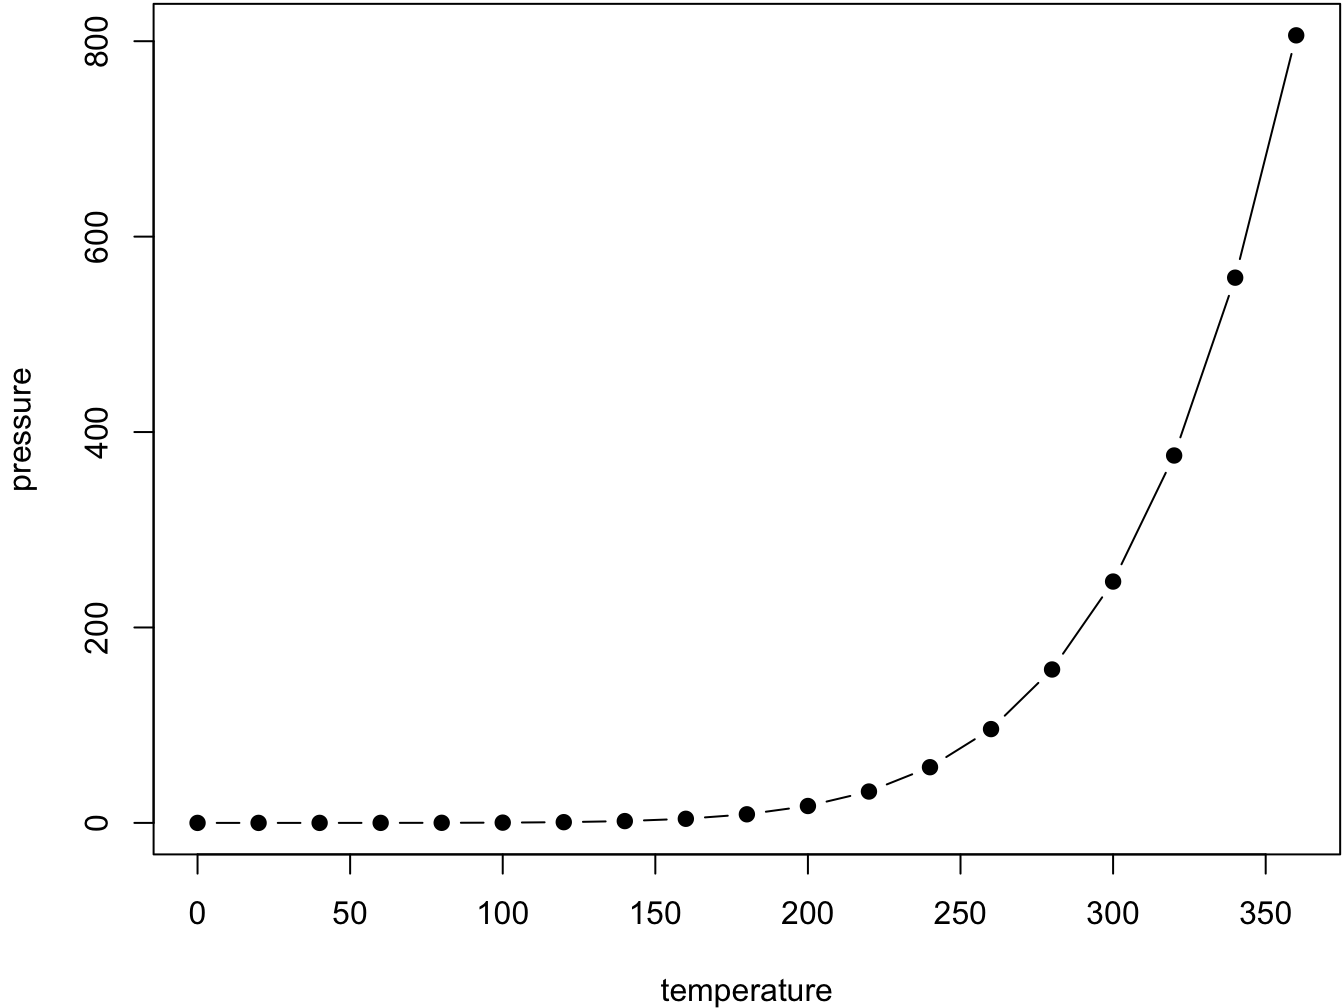
\includegraphics[width=0.8\linewidth]{bookdown-demo_files/figure-latex/nice-fig-1} 

}

\caption{Here is a nice figure!}\label{fig:nice-fig}
\end{figure}

Reference a figure by its code chunk label with the \texttt{fig:} prefix, e.g., see Figure \ref{fig:nice-fig}. Similarly, you can reference tables generated from \texttt{knitr::kable()}, e.g., see Table \ref{tab:nice-tab}.

\begin{Shaded}
\begin{Highlighting}[]
\NormalTok{knitr}\SpecialCharTok{::}\FunctionTok{kable}\NormalTok{(}
  \FunctionTok{head}\NormalTok{(iris, }\DecValTok{20}\NormalTok{), }\AttributeTok{caption =} \StringTok{\textquotesingle{}Here is a nice table!\textquotesingle{}}\NormalTok{,}
  \AttributeTok{booktabs =} \ConstantTok{TRUE}
\NormalTok{)}
\end{Highlighting}
\end{Shaded}

\begin{table}

\caption{\label{tab:nice-tab}Here is a nice table!}
\centering
\begin{tabular}[t]{rrrrl}
\toprule
Sepal.Length & Sepal.Width & Petal.Length & Petal.Width & Species\\
\midrule
5.1 & 3.5 & 1.4 & 0.2 & setosa\\
4.9 & 3.0 & 1.4 & 0.2 & setosa\\
4.7 & 3.2 & 1.3 & 0.2 & setosa\\
4.6 & 3.1 & 1.5 & 0.2 & setosa\\
5.0 & 3.6 & 1.4 & 0.2 & setosa\\
\addlinespace
5.4 & 3.9 & 1.7 & 0.4 & setosa\\
4.6 & 3.4 & 1.4 & 0.3 & setosa\\
5.0 & 3.4 & 1.5 & 0.2 & setosa\\
4.4 & 2.9 & 1.4 & 0.2 & setosa\\
4.9 & 3.1 & 1.5 & 0.1 & setosa\\
\addlinespace
5.4 & 3.7 & 1.5 & 0.2 & setosa\\
4.8 & 3.4 & 1.6 & 0.2 & setosa\\
4.8 & 3.0 & 1.4 & 0.1 & setosa\\
4.3 & 3.0 & 1.1 & 0.1 & setosa\\
5.8 & 4.0 & 1.2 & 0.2 & setosa\\
\addlinespace
5.7 & 4.4 & 1.5 & 0.4 & setosa\\
5.4 & 3.9 & 1.3 & 0.4 & setosa\\
5.1 & 3.5 & 1.4 & 0.3 & setosa\\
5.7 & 3.8 & 1.7 & 0.3 & setosa\\
5.1 & 3.8 & 1.5 & 0.3 & setosa\\
\bottomrule
\end{tabular}
\end{table}

You can write citations, too. For example, we are using the \textbf{bookdown} package \citep{R-bookdown} in this sample book, which was built on top of R Markdown and \textbf{knitr} \citep{xie2015}.

\hypertarget{about-us}{%
\chapter{About Us}\label{about-us}}

about us section

\hypertarget{why-choose-mban-program-at-ross}{%
\chapter{Why Choose MBAn Program at Ross?}\label{why-choose-mban-program-at-ross}}

add details

\hypertarget{expected-values-gained-from-investing-your-time-and-money}{%
\section{Expected values gained from investing your time and money}\label{expected-values-gained-from-investing-your-time-and-money}}

\hypertarget{coursework}{%
\section{Coursework}\label{coursework}}

\hypertarget{career-resources}{%
\section{Career resources}\label{career-resources}}

\hypertarget{long-term-gains}{%
\section{Long-term gains}\label{long-term-gains}}

\hypertarget{career-choices}{%
\chapter{Career Choices}\label{career-choices}}

\hypertarget{expected-career-outcomes}{%
\section{Expected Career Outcomes}\label{expected-career-outcomes}}

\hypertarget{consulting}{%
\subsection{Consulting}\label{consulting}}

\hypertarget{product-management}{%
\subsection{Product Management}\label{product-management}}

\hypertarget{data-analyst}{%
\subsection{Data Analyst}\label{data-analyst}}

\hypertarget{company-search-process}{%
\section{Company Search Process}\label{company-search-process}}

\hypertarget{deciding-dream}{%
\subsection{Deciding Dream}\label{deciding-dream}}

\hypertarget{networking}{%
\subsection{Networking}\label{networking}}

\hypertarget{list-of-companies}{%
\subsection{List of Companies}\label{list-of-companies}}

\hypertarget{recruiting-process}{%
\chapter{Recruiting Process}\label{recruiting-process}}

\hypertarget{resume-preparation-process}{%
\section{Resume preparation process}\label{resume-preparation-process}}

\hypertarget{whats-in-your-toolbox}{%
\subsection{What's in your ``Toolbox''}\label{whats-in-your-toolbox}}

\hypertarget{what-resources-does-oym-provide}{%
\subsection{What resources does OYM provide?}\label{what-resources-does-oym-provide}}

\hypertarget{list-and-links-to-useful-resources-to-look-out-for}{%
\subsection{List and links to useful resources to look out for}\label{list-and-links-to-useful-resources-to-look-out-for}}

\hypertarget{interview-preparation-process}{%
\section{Interview preparation process}\label{interview-preparation-process}}

\hypertarget{sample-questions}{%
\subsection{Sample questions}\label{sample-questions}}

\hypertarget{mock-interviews}{%
\subsection{Mock interviews}\label{mock-interviews}}

\hypertarget{interview-prep-books-reaching-out-to-full-time-mbaconsulting-club-and-mm-who-has-experience}{%
\subsection{Interview Prep books (reaching out to full-time mba(consulting club) and mm (who has experience))}\label{interview-prep-books-reaching-out-to-full-time-mbaconsulting-club-and-mm-who-has-experience}}

\hypertarget{expected-timeline-and-plan}{%
\section{Expected timeline and plan}\label{expected-timeline-and-plan}}

\hypertarget{schedule-for-different-industries-recruiting-practices}{%
\subsection{Schedule for different industries recruiting practices}\label{schedule-for-different-industries-recruiting-practices}}

\hypertarget{deadlines-to-give-yourself-to-be-prepared-and-proactive}{%
\subsection{Deadlines to give yourself to be prepared and proactive}\label{deadlines-to-give-yourself-to-be-prepared-and-proactive}}

\hypertarget{time-management-for-balancing-recruiting-and-classes-simultaneously}{%
\subsection{Time management for balancing recruiting and classes simultaneously}\label{time-management-for-balancing-recruiting-and-classes-simultaneously}}

\hypertarget{challenges-for-international-students.}{%
\chapter{Challenges for International students.}\label{challenges-for-international-students.}}

\hypertarget{sponsorship}{%
\section{Sponsorship}\label{sponsorship}}

\hypertarget{h1b-process}{%
\section{H1B process}\label{h1b-process}}

\hypertarget{resources}{%
\section{Resources}\label{resources}}

\hypertarget{mban-career-handbook}{%
\chapter{MBAn Career Handbook}\label{mban-career-handbook}}

\hypertarget{executive-summary}{%
\subsection{Executive summary}\label{executive-summary}}

\begin{quote}
This handbook is for current and future MBAn students to understand how the program works, what the targeted jobs are, and how to prepare for recruiting processes. The handbook will first begin with an overview of the MBAn program, describing different resources available from the Ross experience, classes you may take, and the skills gained from it. Following this introduction, we will transition into the main section of the book, detailing career outcomes available to MBAn students, driven by research from other school's Business Analytics program, the CDO resources, and experiences from former Master of Management students that have moved onto careers. We will introduce techniques for going through career exploration independently while utilizing the guide. Next will be a chapter focusing on the overall recruiting process for the discussed careers and how MBAn students can prepare and plan for networking, applications, and interviews. We will accumulate best practices for resumes, cover letters, and interviews. A final section will be included detailing supportive resources for the challenges international students face when searching for careers in the U.S. and globally, including a dynamic list of companies that offer sponsorship. We recognize research and resources our team is able to provide over the next few weeks is non-exhaustive, but we hope for this handbook to be a baseline for future students of this program and can live on and be updated in the future as the Master of Business Analytics Graduates enter the workforce and find success in their careers.
\end{quote}

\hypertarget{why-do-we-choose-mban-at-ross}{%
\subsection{Why do we choose MBAn at Ross?}\label{why-do-we-choose-mban-at-ross}}

\begin{itemize}
\tightlist
\item
  Expected values gained from investing your time and money
\item
  Coursework
\item
  Career resources
\item
  Long-term gains
\end{itemize}

\hypertarget{career-choices-1}{%
\subsection{Career choices}\label{career-choices-1}}

\begin{itemize}
\tightlist
\item
  Expected career outcomes after MBAn (Things to prepare for the specific roles) TBD

  \begin{itemize}
  \tightlist
  \item
    Consulting
  \item
    Product Management
  \item
    Data Analyst (Business Analyst)
  \end{itemize}
\item
  Company searching process

  \begin{itemize}
  \tightlist
  \item
    Decide your own dream direction and dream companies appropriate for you most(LAMP list)
  \item
    Be brave to reaching out and talking to people (alumni \& other school's business analytics), insights from alumni in analytical roles \& CDO
  \item
    List of companies for these roles, including whether to offer sponsorship or not
  \end{itemize}
\end{itemize}

\hypertarget{recruiting-process-1}{%
\subsection{Recruiting process}\label{recruiting-process-1}}

\begin{itemize}
\tightlist
\item
  Resume preparation process

  \begin{itemize}
  \tightlist
  \item
    What's in your ``Toolbox''
  \item
    What resources does OYM provide?
  \item
    List and links to useful resources to look out for
  \end{itemize}
\item
  Interview preparation process

  \begin{itemize}
  \tightlist
  \item
    Sample questions
  \item
    Mock interviews
  \item
    Interview Prep books (reaching out to full-time mba(consulting club) and mm (who has experience))
  \item
    Expected timeline and plan
  \item
    Schedule for different industries recruiting practices
  \item
    Deadlines to give yourself to be prepared and proactive
  \item
    Time management for balancing recruiting and classes simultaneously
  \end{itemize}
\end{itemize}

\hypertarget{challenges-for-international-students}{%
\subsection{Challenges for International students}\label{challenges-for-international-students}}

\begin{enumerate}
\def\labelenumi{\arabic{enumi}.}
\tightlist
\item
  Sponsorship
\item
  H1B process
\item
  Resources
\end{enumerate}

\hypertarget{pointers-to-work-on}{%
\subsubsection{Pointers to work on}\label{pointers-to-work-on}}

\begin{itemize}
\tightlist
\item
  Business Analytics is domain independent.
\item
  Keep track of references.
\item
  Use glassdoor as a reference.
\item
  Taking in first hand references from Alum.
\end{itemize}

  \bibliography{book.bib,packages.bib}

\end{document}
